\documentclass[14pt,a4paper]{extarticle}

\usepackage[utf8]{inputenc}
\usepackage[T2A]{fontenc}
\usepackage{amssymb,amsmath,mathrsfs,amsthm}
\usepackage[russian]{babel}
\usepackage{graphicx}
\usepackage[footnotesize]{caption2}
\usepackage{indentfirst}
\usepackage{multicol}
\usepackage{listings}
\usepackage{float}
\usepackage{url}
\usepackage{amsmath}

\usepackage{enumitem}

%\usepackage[ruled,section]{algorithm}
%\usepackage[noend]{algorithmic}
%\usepackage[all]{xy}
\usepackage{booktabs}
\usepackage{graphicx}
\usepackage[table,xcdraw]{xcolor}
\usepackage{tcolorbox}

%Библиотека для блок-схем
\usepackage{tikz}
\usetikzlibrary{shapes,arrows}

% Параметры страницы
\textheight=24cm
\textwidth=16cm
\oddsidemargin=5mm
\evensidemargin=-5mm
\marginparwidth=36pt
\topmargin=-1cm
\footnotesep=3ex
%\flushbottom
\raggedbottom
\tolerance 3000
% подавить эффект "висячих стpок"
\clubpenalty=10000
\widowpenalty=10000
%\renewcommand{\baselinestretch}{1.1}
\renewcommand{\baselinestretch}{1.5} %для печати с большим интервалом

\newcommand{\angstrom}{\mbox{\normalfont\AA}}

\newtheorem{definition}{Определение} % задаём выводимое слово (для определений)
\newtheorem{example}{Замечание} % задаём выводимое слово (для определений)
\newtheorem{theorem}{Теорема} % задаём выводимое слово (для определений)
\newtheorem{proposition}{Утверждение} % задаём выводимое слово (для определений)
\newtheorem{construction}{Конструкция} % задаём выводимое слово (для определений)

\DeclareMathOperator*{\sgn}{sgn}
\DeclareMathOperator*{\var}{var}
\DeclareMathOperator*{\cov}{cov}
\DeclareMathOperator*{\law}{Law}

\newcommand{\1}{\mathbbm{1}}
\newcommand{\R}{\mathbb{R}}
\newcommand{\N}{\mathbb{N}}
\newcommand{\Z}{\mathbb{Z}}
\renewcommand{\P}{\mathbb{P}}
\newcommand{\E}{\mathbb{E}}

\newcommand{\independent}{\perp\!\!\!\!\perp}

\newcommand\cA{{\cal A}}
\newcommand\cE{{\cal E}}
\newcommand\cC{{\cal C}}
\newcommand\cF{{\cal F}}
\newcommand\cG{{\cal G}}
\newcommand\cK{{\cal K}}
\newcommand\cL{{\cal L}}
\newcommand\cB{{\cal B}}
\newcommand\cN{{\cal N}}
\newcommand\cM{{\cal M}}
\newcommand\cX{{\cal X}}
\newcommand\cD{{\cal D}}
\newcommand\cR{{\cal R}}
\newcommand\cP{{\cal P}}
\newcommand\cQ{{\cal Q}}
\newcommand\cS{{\cal S}}
\newcommand\cT{{\cal T}}
\newcommand\cV{{\cal V}}
\newcommand\cZ{{\cal Z}}

\newcommand{\textProposition}    {Предложение}
\newcommand{\textTask}    {Задача}

\begin{document}

\begin{center}
    {Всеволод Заостровский, 409 группа}\\
    {\bfseries Отчёт по задаче '' Метод Фурье для уравнения теплопроводности для двумерного оператора Лапласа''.\\}
    \vspace{1cm}
\end{center}

\tableofcontents

\section{Постановка задачи.} \label{diffeq1}
Необходимо решить уравнение:
\begin{equation*} 
    u_t(t, x) = u_{xx}(t, x, y) + u_{yy}(t, x, y) + f(t, x, y).
\end{equation*}
Будем считать, что $0 \leq t,x,y \leq 1$. В моём варианте, краевые условия:
\begin{align*} 
    &u(t, x, y) \big| _{(x ,y) \in \partial \Omega} = 0, \quad \Omega = [0,1] \times [0,1]. \\
    &u(0, x, y) = u^0(x, y), \quad (x, y) \in \Omega. 
\end{align*}


% \section{Решение дифференциального уравнения (для тестов).}\label{solution}
% Будем искать решение в виде $u(t, x, y) = T(t) X(x) Y(y)$. С учетом краевых условий, получим:
% \begin{align*} 
%     & u(t, x, 0) = T(t) X(x) Y(0) = 0 \Rightarrow Y(0) = 0, \\
%     & u(t, x, 1) = T(t) X(x) Y(1) = 0 \Rightarrow Y(1) = 0, \\
%     & u(t, 0, y) = T(t) X(0) Y(y) = 0 \Rightarrow X(0) = 0, \\
%     & u(t, 1, y) = T(t) X(1) Y(y) = 0 \Rightarrow X(1) = 0.
% \end{align*}
% Разрешим уравнение с учетом $u(t, x) = T(t) X(x) Y(y)$:
% \begin{align*} 
%     & T' X Y = T X'' Y + T X Y'', \\
%     & \frac{X''}{X} + \frac{Y''}{Y} = \frac{T'}{T} = -\lambda.
% \end{align*}



\section{Дискретизация дифференциального уравнения.} \label{scheme1}
Исходной задаче (см. раздел \ref{diffeq1}) предлагается сопоставлять следующую схему:
\begin{align*}
    &\frac{u_{i, j}^{n+1} - u_{i, j}^n}{\tau} = \frac{u_{i+1, j}^{n+1} - 2 u_{i, j}^{n+1} + u_{i-1, j}^{n+1}}{h_X^2} + 
    \frac{u_{i, j+1}^{n+1} - 2 u_{i, j}^{n+1} + u_{i, j-1}^{n+1}}{h_Y^2} + f(t_{n}, x_{i+1}, y_{j+1}), \\
    & i = 1 \ldots N_X, \quad j = 1 \ldots N_Y, \quad n = 1 \ldots N-1.
\end{align*}
Краевые условия примут вид:
\begin{align*} 
    &\forall i, j, n \in \{0, 1, \ldots N_X\}\times\{0, 1, \ldots N_Y\}\times\{0, 1, \ldots N\} ,\\
    &u^n_h(1, j) = u^n_h(0, j) = u^n_h{(i, 0)} = u^n_h{(i, 1)} = 0, \\
    &u^0_h{(i, j)} = u^0_h(i, j). 
\end{align*}
\section{Аппроксимация на решении.}
Разложим значения решения в ряд Тейлора:
\begin{align*}
    u(t_n, x_{i+1}, y_j) &= u(t_n, x_{i}, y_j) +    h_X u_x(t_n, x_{i}, y_j) 
    + \frac{h_X^2}{2}u_{xx}(t_n, x_{i}, y_j) \\ &+\frac{h_X^3}{6}u_{xxx}(t_n, x_{i}, y_j) +    \frac{h_X^4}{24}u_{xxxx}(t_n, x_{i}, y_j) + O(h_X^5) \\
    u(t_n, x_{i-1}, y_{j}) &= u(t_n, x_{i}, y_j) - h_X u_x(t_n, x_{i}, y_j) 
    + \frac{h_X^2}{2}u_{xx}(t_n, x_{i}, y_j) \\ &-   \frac{h_X^3}{6}u_{xxx}(t_n, x_{i}, y_j) +    \frac{h_X^4}{24}u_{xxxx}(t_n, x_{i}, y_j) + O(h_X^5) \\
    u(t_n, x_{i}, y_{j+1}) &= u(t_n, x_{i}, y_j) +    h_Y u_y(t_n, x_{i}, y_j) 
    + \frac{h_Y^2}{2}u_{yy}(t_n, x_{i}, y_j) \\ &+ \frac{h_Y^3}{6}u_{yyy}(t_n, x_{i}, y_j) +    \frac{h_Y^4}{24}u_{yyyy}(t_n, x_{i}, y_j) + O(h_Y^5) \\
    u(t_n, x_{i}, y_{j-1}) &= u(t_n, x_{i}, y_j) - h_Y u_y(t_n, x_{i}, y_j) 
    + \frac{h_Y^2}{2}u_{yy}(t_n, x_{i}, y_j) \\ &- \frac{h_Y^3}{6}u_{yyy}(t_n, x_{i}, y_j) +    \frac{h_Y^4}{24}u_{yyyy}(t_n, x_{i}, y_j) + O(h_Y^5) \\
    u(t_{n+1}, x_i, y_j) &= u(t_{n}, x_i, y_j)+ \tau u_x(t_{n}, x_i, y_j) + \frac{\tau^2}{2}u_{tt}(t_n, x_i, y_j) + \frac{\tau^3}{6}u_{ttt}(t_n, x_i, y_j) \\
    &+ \frac{\tau^4}{24}u_{tttt}(t_n, x_i, y_j) + O(\tau^5) \\
    u(t_{n-1}, x_m) &= u(t_{n}, x_i, y_j)- \tau u_x(t_{n}, x_i, y_j) + \frac{\tau^2}{2}u_{tt}(t_n, x_i, y_j) - \frac{\tau^3}{6}u_{ttt}(t_n, x_i, y_j) \\
    &+ \frac{\tau^4}{24}u_{tttt}(t_n, x_i, y_j) + O(\tau^5) \\
\end{align*}
Отсюда имеем:
\begin{align*}
    \frac{u_{i, j}^{n+1} - u_{i, j}^n}{\tau} &=   \frac{u(t_{n+1}, x_i, y_j) - u(t_n, x_i, y_j)}{\tau} = u_t(t_{n}, x_i, y_j) \\
    &+\frac{\tau}{2}u_{tt}(t_n, x_{i}, y_j) + \frac{\tau^2}{6}u_{ttt}(t_n, x_{i}, y_j)+ \frac{\tau^3}{24}u_{tttt}(t_n, x_{i}, y_j) + O(\tau^4) \\
    \frac{u_{i+1, j}^{n+1} - 2 u_{i, j}^{n+1} + u_{i-1, j}^{n+1}}{h_X^2} &= \frac{u(t_{n+1}, x_{i+1}, y_j) - 2 u(t_{n+1}, x_{i}, y_j) + u(t_{n+1}, x_{i-1}, y_j)}{h_X^2} = \\
    &= u_{xx}(t_n, x_{i}, y_j) + \frac{h_X^2}{12}u_{xxxx}(t_n, x_{i}, y_j) + O(h_X^4)\\
    \frac{u_{i, j+1}^{n+1} - 2 u_{i, j}^{n+1} + u_{i, j-1}^{n+1}}{h_Y^2} &=\frac{u(t_{n+1}, x_{i}, y_{j+1}) - 2 u(t_{n+1}, x_{i}, y_j) + u(t_{n+1}, x_{i}, y_{j-1})}{h_Y^2} = \\
    &= u_{yy}(t_n, x_{i}, y_j) + \frac{h_Y^2}{12}u_{yyyy}(t_n, x_{i}, y_j) + O(h_Y^4)
\end{align*}
Подставив эти выражения в дифференциальное уравнение, получим:
\begin{align*}
    &||\frac{u_{i, j}^{n+1} - u_{i, j}^n}{\tau} - \frac{u_{i+1, j}^{n+1} - 2 u_{i, j}^{n+1} + u_{i-1, j}^{n+1}}{h_X^2} - 
    \frac{u_{i, j+1}^{n+1} - 2 u_{i, j}^{n+1} + u_{i, j-1}^{n+1}}{h_Y^2} - f(t_{n}, x_{i+1}, y_{j+1})|| = \\
    &= ||- u_{xx}(t_n, x_{i}, y_j) - u_{yy}(t_n, x_{i}, y_j) + u_t(t_{n}, x_i, y_j) - f(t_{n}, x_{i+1}, y_{j+1}) + O(\ldots)||=\\ &=
     O(\tau + h_X^2 + h_Y^2).
\end{align*}
С учетом того, что начальные условия даны точно и, очевидно, $|f(t_n, x_i, y_j) - f_{i,j}^n| \rightarrow 0$, получаем, что порядок аппроксимации на решении 
данной схемы составляет $O(\tau + h_X^2 + h_Y^2)$.

\section{Разложение функции в двумерный ряд Фурье}
Функцию $u(x, y) \in C^{\infty}[0, 1]^2$ можно разложить в ряд Фурье,
взяв синусы в качестве базисных функций:
\begin{equation*}
    u(x) = \sum_{m, n = 1}^{\infty} c_{mn} \sin {\pi m x} \sin {\pi n y}.
\end{equation*}
\par
Перейдём к рассмотрению конечного числа узлов. Выпишем условия на сетку:
\begin{align*}
     & u_{ij} := u(x_i, y_j), \quad x_i = \frac{i}{N_X}, \quad y_j := \frac{j}{N_Y}\\
     & u_{ij} = \sum_{n, m = 1}^{N_X-1, N_Y-1} c_{nm} \phi_i^{(n)} \psi_j^{(m)},                                    \\
     & \phi_i^{(n)} := \sin{\pi n i h_X} = \sin\left(\frac{\pi n i}{N_X}\right) \\
     & \psi_j^{(m)} := \sin{\pi m j h_Y} = \sin\left(\frac{\pi m j}{N_Y}\right) \\
     & \phi^n := (\phi_1^n ... \phi_{N_X-1}^n), \quad \psi^m := (\psi_1^m ... \psi_{N_Y-1}^m).
\end{align*}
% Убедимся, что указанные функции ортогональны относительно скалярного произведения
% ${(\phi^k, \phi^j) = \sum_{m = 1}^{N - 1}\phi_m^k \phi_m^j h}$:

% \begin{align*}
%      & (\phi^k, \phi^j) = \sum_{m = 1}^{N - 1} \phi_m^k \phi_m^j h
%     = \sum_{m = 1}^{N - 1} \sin{\pi k (\frac{-h}{2} + m h)} \sin{\pi j (\frac{-h}{2} + m h)} h                                   \\
%      & = \frac{1}{2} \sum_{m = 1}^{N - 1} [ \cos{(\pi h (m - \frac{1}{2})(k - j))} - \cos{(\pi h (m - \frac{1}{2})(k + j))} ] h.
% \end{align*}

% Заметим, что при $\alpha \neq 0$ справедливо:
% \begin{align*}
%      & \sum_{m = 1}^{N - 1} \cos(\alpha m - \frac{\alpha}{2}) = Re\sum_{m = 1}^{N - 1} e^{i (\alpha m - \frac{\alpha}{2})}
%     = Re \frac{e^{\frac{i \alpha}{2}(e^{i \alpha (N - 1)} - 1)}}{e^{i \alpha - 1}}
%     = \frac{Im [-1 + e^{i (N - 1) \alpha}]}{2 \sin(\alpha/2)}                                                              \\
%      & = \frac{\sin{(N - 1) \alpha}}{2 \sin(\alpha/2)}.
% \end{align*}

% Отсюда при $k \neq j$:

% \begin{align*}
%      & (\phi^k, \phi^j)
%     = \frac{1}{2} \sum_{m = 1}^{N - 1} [ \cos{(\pi h (m - \frac{1}{2})(k - j))} - \cos{(\pi h (m - \frac{1}{2})(k + j))} ] h                        \\
%      & = h \left[ \frac{\sin{(N - 1) \pi h (k - j)}}{4 \sin(\pi h (k - j)/2)} - \frac{\sin{(N - 1) \pi h (k + j)}}{4 \sin(\pi h (k + j)/2)} \right] \\
%      & = h \left[ \frac{\sin(\pi (k - j) - \pi h (k - j))}{4 \sin(\pi h (k - j)/2)}
%     - \frac{\sin(\pi (k + j) - \pi h (k + j))}{4 \sin(\pi h (k + j)/2)}\right]                                                                      \\
%      & = h \left[ \frac{(-1)^{k-j}\sin(\pi h (k - j))}{4 \sin(\pi h (k - j)/2)}
%     - \frac{(-1)^{k+j}\sin(\pi h (k + j))}{4 \sin(\pi h (k + j)/2)}\right]                                                                          \\
%      & = \frac{h}{2} [(-1)^{k-j}\sin(\pi h (k - j)/2) - (-1)^{k+j}\sin(\pi h (k + j)/2)] = 0.
% \end{align*}

% В ином случае,
% \begin{align*}
%      & (\phi^k, \phi^k)
%     = \frac{1}{2} \sum_{m = 1}^{N - 1} [ \cos{(\pi h (m - \frac{1}{2})(k - k))} - \cos{(\pi h (m - \frac{1}{2})(k + k))} ] h \\
%      & = h \left[ \frac{N - 1}{2} - \frac{\sin{2 (N - 1) \pi h k}}{4 \sin(\pi h k)} \right]
%     = \frac{2 N - 1}{4} \frac{2}{2 N - 1} = \frac{1}{2}.
% \end{align*}

% Отсюда, очевидно, система функций $\psi_{ij}^{mn} := \phi_i^m \phi_j^n $. \par
Искать коэффициенты будем по следующему алгоритму:
\begin{enumerate}
    \item Вычислим матрицу $u_{ij}:= u(x_i, y_j)$.
    \item Зафиксируем $j$ и разложим $u^j(i) := u_{ij}$ в одномерный ряд Фурье:
          \begin{equation*}
              u^j(i) = \sum _{n = 1}^{N_X - 1} \phi_i^{(n)} d_n^j.
          \end{equation*}
          Полученные коэффициенты запишем в новую матрицу.
    \item По вектору $d_n^j$ восстановим коэффициенты $c_{nm}$ посредством ещё одного разложения в ряд:
          \begin{equation*}
              d_n^j = \sum _{m = 1}^{N_Y - 1} c_{nm} \psi_j^m.
          \end{equation*}
\end{enumerate}



\section{Алгоритм численного решения.}
\subsection{Общая идея решения.}
Запишем схему в виде:
\begin{align*} 
    &- \frac{u_{i+1, j}^{n+1} - 2 u_{i, j}^{n+1} + u_{i-1, j}^{n+1}}{h_X^2} - \frac{u_{i, j+1}^{n+1} - 2 u_{i, j}^{n+1} + u_{i, j-1}^{n+1}}{h_Y^2} + \frac{u_{i, j}^{n+1}}{\tau} = \\&= 
    \frac{u_{i, j}^n}{\tau} + f(t_{n}, x_{i+1}, y_{j+1}).
\end{align*}
Фактически, это трехмерная система уравнений. Первый слой $u_{i, j}^{0} \big|^{n+1} _{0 \leq i, j, \leq 1}$ 
известен из начального условия. Если, располагая этими данными, удастся вычислить следующий слой, то, повторяя процесс шаг за шагом мы вычислим всю матрицу. Это возможно, поскольку, если считать $u^{n} =\text{const}$ схема выше представляет собой систему линейных уравнений относительно $u_{i, j}^{n+1}$. 
Далее подробно описан процесс нахождения сети методом Фурье.
\subsection{Получение $n + 1$ слоя из $n$-го.}
Если нам известен слой $u_{i, j}^{n} \big|^{n = \text{const}} _{0 \leq i, j, \leq 1}$, то для определения слоя $u_{i, j}^{n} \big|^{n+1} _{0 \leq i, j, \leq 1}$ необходимо решить систему уравнений выше. Проще всего сделать это методом Фурье. Заметим, что эта система образует схему для дифференциальной задачи:
\begin{align*} 
    & - \Delta u(x, y) + p u(x , y) = \hat f(x, y), 
\end{align*}
где $p = \frac{1}{\tau}$, а $\hat f = \frac{u}{\tau} + f(x, y)$.

Функции $u(x, y), f(x, y) \in C^{\infty}_0[0, 1]^2$ можно разложить в ряд Фурье,
взяв синусы в качестве базисных функций:
\begin{align*}
    u(x, y) &= \sum_{n, m = 1}^{\infty} \hat c_{nm} \phi ^{(n)}(x) \psi ^{(m)}(y), \\
    \hat f(x, y) &= \sum_{n, m = 1}^{\infty} \hat d_{nm} \phi ^{(n)}(x) \psi ^{(m)}(y),
\end{align*}
где
\begin{align*}
    \phi ^{(n)}(x) = \sin {\pi n x}, \quad \psi ^{(m)}(y) = \sin {\pi m y}.
\end{align*}
Перейдем в дискретное время:
\begin{align*}
    u(x_i, y_j) = u_h(i, j) &= \sum_{n, m = 1}^{N_X-1, N_Y-1} c_{nm} \phi ^{(n)}_i \psi ^{(m)}_j, \\
    \hat f(x_i, y_j) = \hat f_h(i, j) &= \sum_{n, m = 1}^{N_X-1, N_Y-1} d_{nm} \phi ^{(n)}_i \psi ^{(m)}_j,
\end{align*}
где
\begin{align*}
    \phi _{i}^{(n)} := \phi ^{(n)}(x_i) = \sin {\pi n i h_X}, \quad 
    \psi _{j}^{(m)} := \psi ^{(m)}(x_j) = \sin {\pi m j h_Y}.
\end{align*}
В отчете по задаче по линейной алгебре (см. директорию "LinAlg") были вычислены собственные значения этой функции для дискретизации оператора Лапласа:
\begin{align*}
    -\Delta _h^X \phi _{i}^{(n)} &= \lambda^X_n \phi _{i}^{(n)}, \quad 
    \lambda^X_n = \frac{4}{h_X^2} \sin ^2\left(\frac{\pi n h_X}{2}\right), \\
    -\Delta _h^Y \psi _{j}^{(m)} &= \lambda^Y_m \psi _{j}^{(m)}, \quad 
    \lambda^Y_m = \frac{4}{h_Y^2} \sin ^2\left(\frac{\pi m h_Y}{2}\right).
\end{align*}
С учетом этого, для схемы 
\begin{align*}
    -\Delta _h^X u_h(i, j) -\Delta _h^Y u_h(i, j) + p u_h(i, i)= \hat f_h(i, j)
\end{align*}
справедливо представление в виде ряда:
\begin{align*}
    -\left(\Delta _h^X + \Delta _h^Y\right) \sum_{n, m = 1}^{N_X-1, N_Y-1} c_{nm} \phi ^{(n)}_i \psi ^{(m)}_j  
    + p \sum_{n, m = 1}^{N_X-1, N_Y-1} c_{nm} \phi ^{(n)}_i \psi ^{(m)}_j =\\
    =   \sum_{n, m = 1}^{N_X-1, N_Y-1} d_{nm} \phi ^{(n)}_i \psi ^{(m)}_j.
\end{align*}
Отсюда, учитывая то, что $\phi ^{(n)}_i$ и $\psi ^{(m)}_j$ --- собственные функции, имеем:
\begin{align*}
    \sum_{n, m = 1}^{N_X-1, N_Y-1} c_{nm} (\lambda^X_n +  \lambda^Y_m + p) \phi ^{(n)}_i \psi ^{(m)}_j  
    = \sum_{n, m = 1}^{N_X-1, N_Y-1} d_{nm} \phi ^{(n)}_i \psi ^{(m)}_j,
\end{align*}
а значит
\begin{align*}
    c_{nm} = \frac{d_{nm}}{\lambda^X_n +  \lambda^Y_m + p}, \quad 1 \leq n \leq N_X-1, \quad 1 \leq m \leq N_Y-1.
\end{align*}
\subsection{Практический алгоритм.}
Решить схему из раздела \ref{scheme1} можно по следующему алгоритму:
\begin{enumerate}
    \item На этапе $G$ известен слой $G: \ u_{i, j}^{G} \big|^{G = \text{const}} _{0 \leq i, j \leq N_x, N_y}$ и все слои до него.
    \item Найдем коэффициенты $d_{nm}$ разложения функции $\hat f(x, y)$ в дискретный ряд Фурье: 
    \begin{align*}
     \frac{u^{G}_{i, j}}{\tau} + f(t_G, x_i, y_j) =: \hat f(x_i, y_j) =: \hat f_h(i, j) &= \sum_{n, m = 1}^{N_X-1, N_Y-1} \hat d_{nm} \phi ^{(n)}_i \psi ^{(m)}_j.
    \end{align*}
    \item Найдем коэффициенты $c_{nm}$ разложения функции $u^{G+1}(x, y)$ в дискретный ряд Фурье: 
    \begin{align*}
    u(t_{G+1}, x_i, y_j) = u_h^{G+1}(i, j) &= \sum_{n, m = 1}^{N_X-1, N_Y-1} c_{nm} \phi ^{(n)}_i \psi ^{(m)}_j,
    \end{align*}
    пользуясь формулой:
    \begin{align*}
    c_{nm} = \frac{ \hat d_{nm}}{\frac{4}{h_X^2} \sin ^2\left(\frac{\pi n h_X}{2}\right)
    +  \frac{4}{h_Y^2} \sin ^2\left(\frac{\pi m h_Y}{2}\right) + \frac{1}{\tau}}, \\
    \quad 1 \leq n \leq N_X-1, \quad 1 \leq m \leq N_Y-1.
    \end{align*}
    \item Вычислить значения 
    $$
    u^{G+1}(i, j) = \sum_{n, m = 1}^{N_X-1, N_Y-1} c_{nm} \phi ^{(n)}_i \psi ^{(m)}_j
    $$ 
    и записать их в соответсвующий слой матрицы решения.
\end{enumerate}
\subsection{Практический алгоритм --- вариант 2.}
Решить схему из раздела \ref{scheme1} можно по следующему алгоритму:
\begin{enumerate}
    \item На этапе $G$ известны коэффициенты Фурье--разложения решения для фиксированного $t_G: \ u_{i, j}^{G} \big|^{G = \text{const}} _{0 \leq i, j, \leq N_x, N_y} = \sum u_{nm}^G \phi ^{(n)}_i \psi ^{(m)}_j$ и все слои до него.
    \item Найдем коэффициенты $d_{nm}$ разложения функции $f(x, y)$ в дискретный ряд Фурье: 
    \begin{align*}
     f(t_G, x_i, y_j)  &= \sum_{n, m = 1}^{N_X-1, N_Y-1} d_{nm} \phi ^{(n)}_i \psi ^{(m)}_j.
    \end{align*}
    \item Тогда коэффициенты Фурье правой части уравнения можно найти по формуле:
    \begin{align*}
     &\hat f(x_i, y_j) = \frac{u^{G}_{i, j}}{\tau} + f(t_G, x_i, y_j) \\
     &\hat f(x_i, y_j) = \frac{1}{\tau} \sum_{n, m = 1}^{N_X-1, N_Y-1}u_{nm}^G \phi ^{(n)}_i \psi ^{(m)}_j  + \sum_{n, m = 1}^{N_X-1, N_Y-1} d_{nm} \phi ^{(n)}_i \psi ^{(m)}_j = \\
     &= \sum_{n, m = 1}^{N_X-1, N_Y-1} \left(\frac{u_{nm}^G}{\tau} + d_{nm}\right) \phi ^{(n)}_i \psi ^{(m)}_j \Rightarrow \hat d_{nm} = \frac{u_{nm}^G}{\tau} + d_{nm}.
    \end{align*}
    \item Найдем коэффициенты $u_{nm}^{G+1}$ разложения функции $u^{G+1}(x, y)$ в дискретный ряд Фурье: 
    \begin{align*}
    u(t_{G+1}, x_i, y_j) = u_h^{G+1}(i, j) &= \sum_{n, m = 1}^{N_X-1, N_Y-1} u_{nm}^{G+1} \phi ^{(n)}_i \psi ^{(m)}_j,
    \end{align*}
    пользуясь формулой:
    \begin{align*}
    u_{nm}^{G+1} = \frac{\frac{u_{nm}^G}{\tau} + d_{nm}}{\frac{4}{h_X^2} \sin ^2\left(\frac{\pi n h_X}{2}\right)
    +  \frac{4}{h_Y^2} \sin ^2\left(\frac{\pi m h_Y}{2}\right) + \frac{1}{\tau}}, \\
    \quad 1 \leq n \leq N_X-1, \quad 1 \leq m \leq N_Y-1.
    \end{align*}
    \item После нахождения всей трехмерной матрицы коэффициентов Фурье, вычислить значения в каждой точке сетки по этой аппроксимации. 
\end{enumerate}
Был реализован этот вариант.
\section{Тесты}
\subsection{Базисные функции.}
При начальном условии вида
  \begin{align*}
     u(0, x, y) = \sin \pi n x \sin \pi m y.
 \end{align*}
 Легко подобрать решение задачи \ref{diffeq1}:
  \begin{align*}
     u(t, x, y) = e^{-\pi^2 (n^2 + m^2)t} \sin \pi n x \sin \pi m y.
 \end{align*}
 Таким образом, можно проверить правильность вычисления коэффициента Фурье: при этом, корректная работа на базисных функциях даёт существенные основания полагать, 
 что и в общем случае программа будет работать корректно. На них же можно вычислить порядок сходимости 
 (ясно, что домножение на произведение синусов происходит в самом конце и сходимость не испортит). Рассматриваются $1 \leq n, m \leq 2$. Результаты представлены 
 на графиках \ref{tbf11}--\ref{tbf22}.
 \begin{figure}
    \centering
    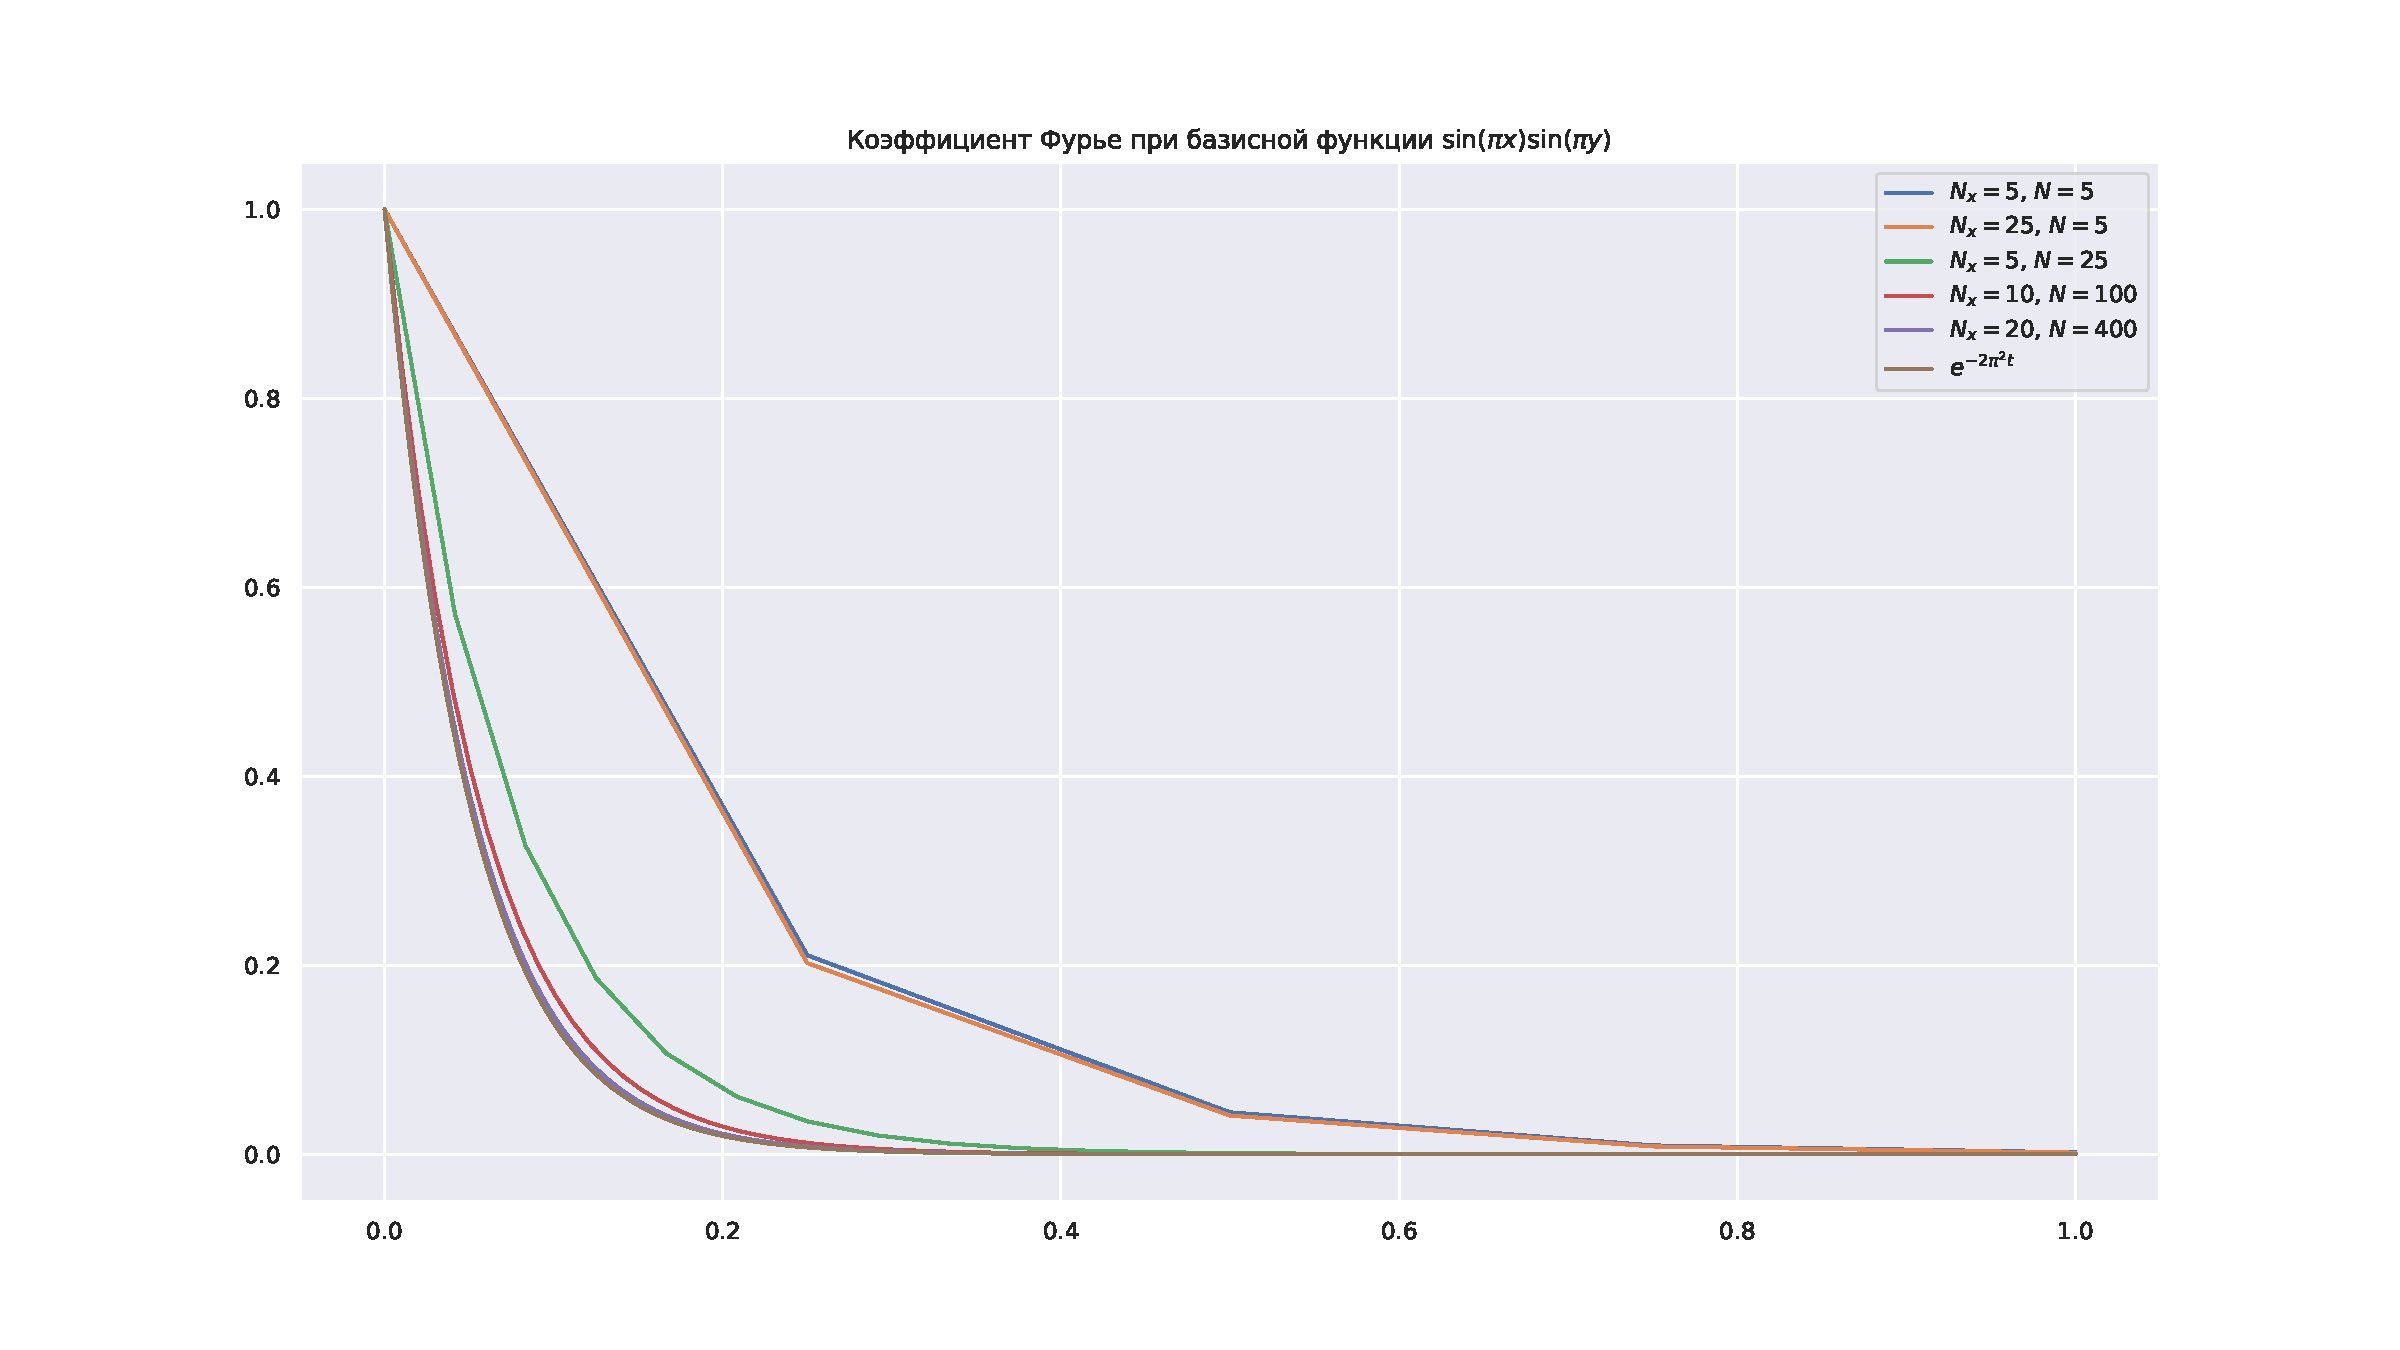
\includegraphics[scale=0.4]{figs/11bf_test.pdf}
    \caption{Задача \ref{diffeq1} при $f = 0$, $u(0, x, y) = \sin \pi n x \sin \pi m y$ }
    \label{tbf11}
\end{figure}
\begin{figure}
    \centering
    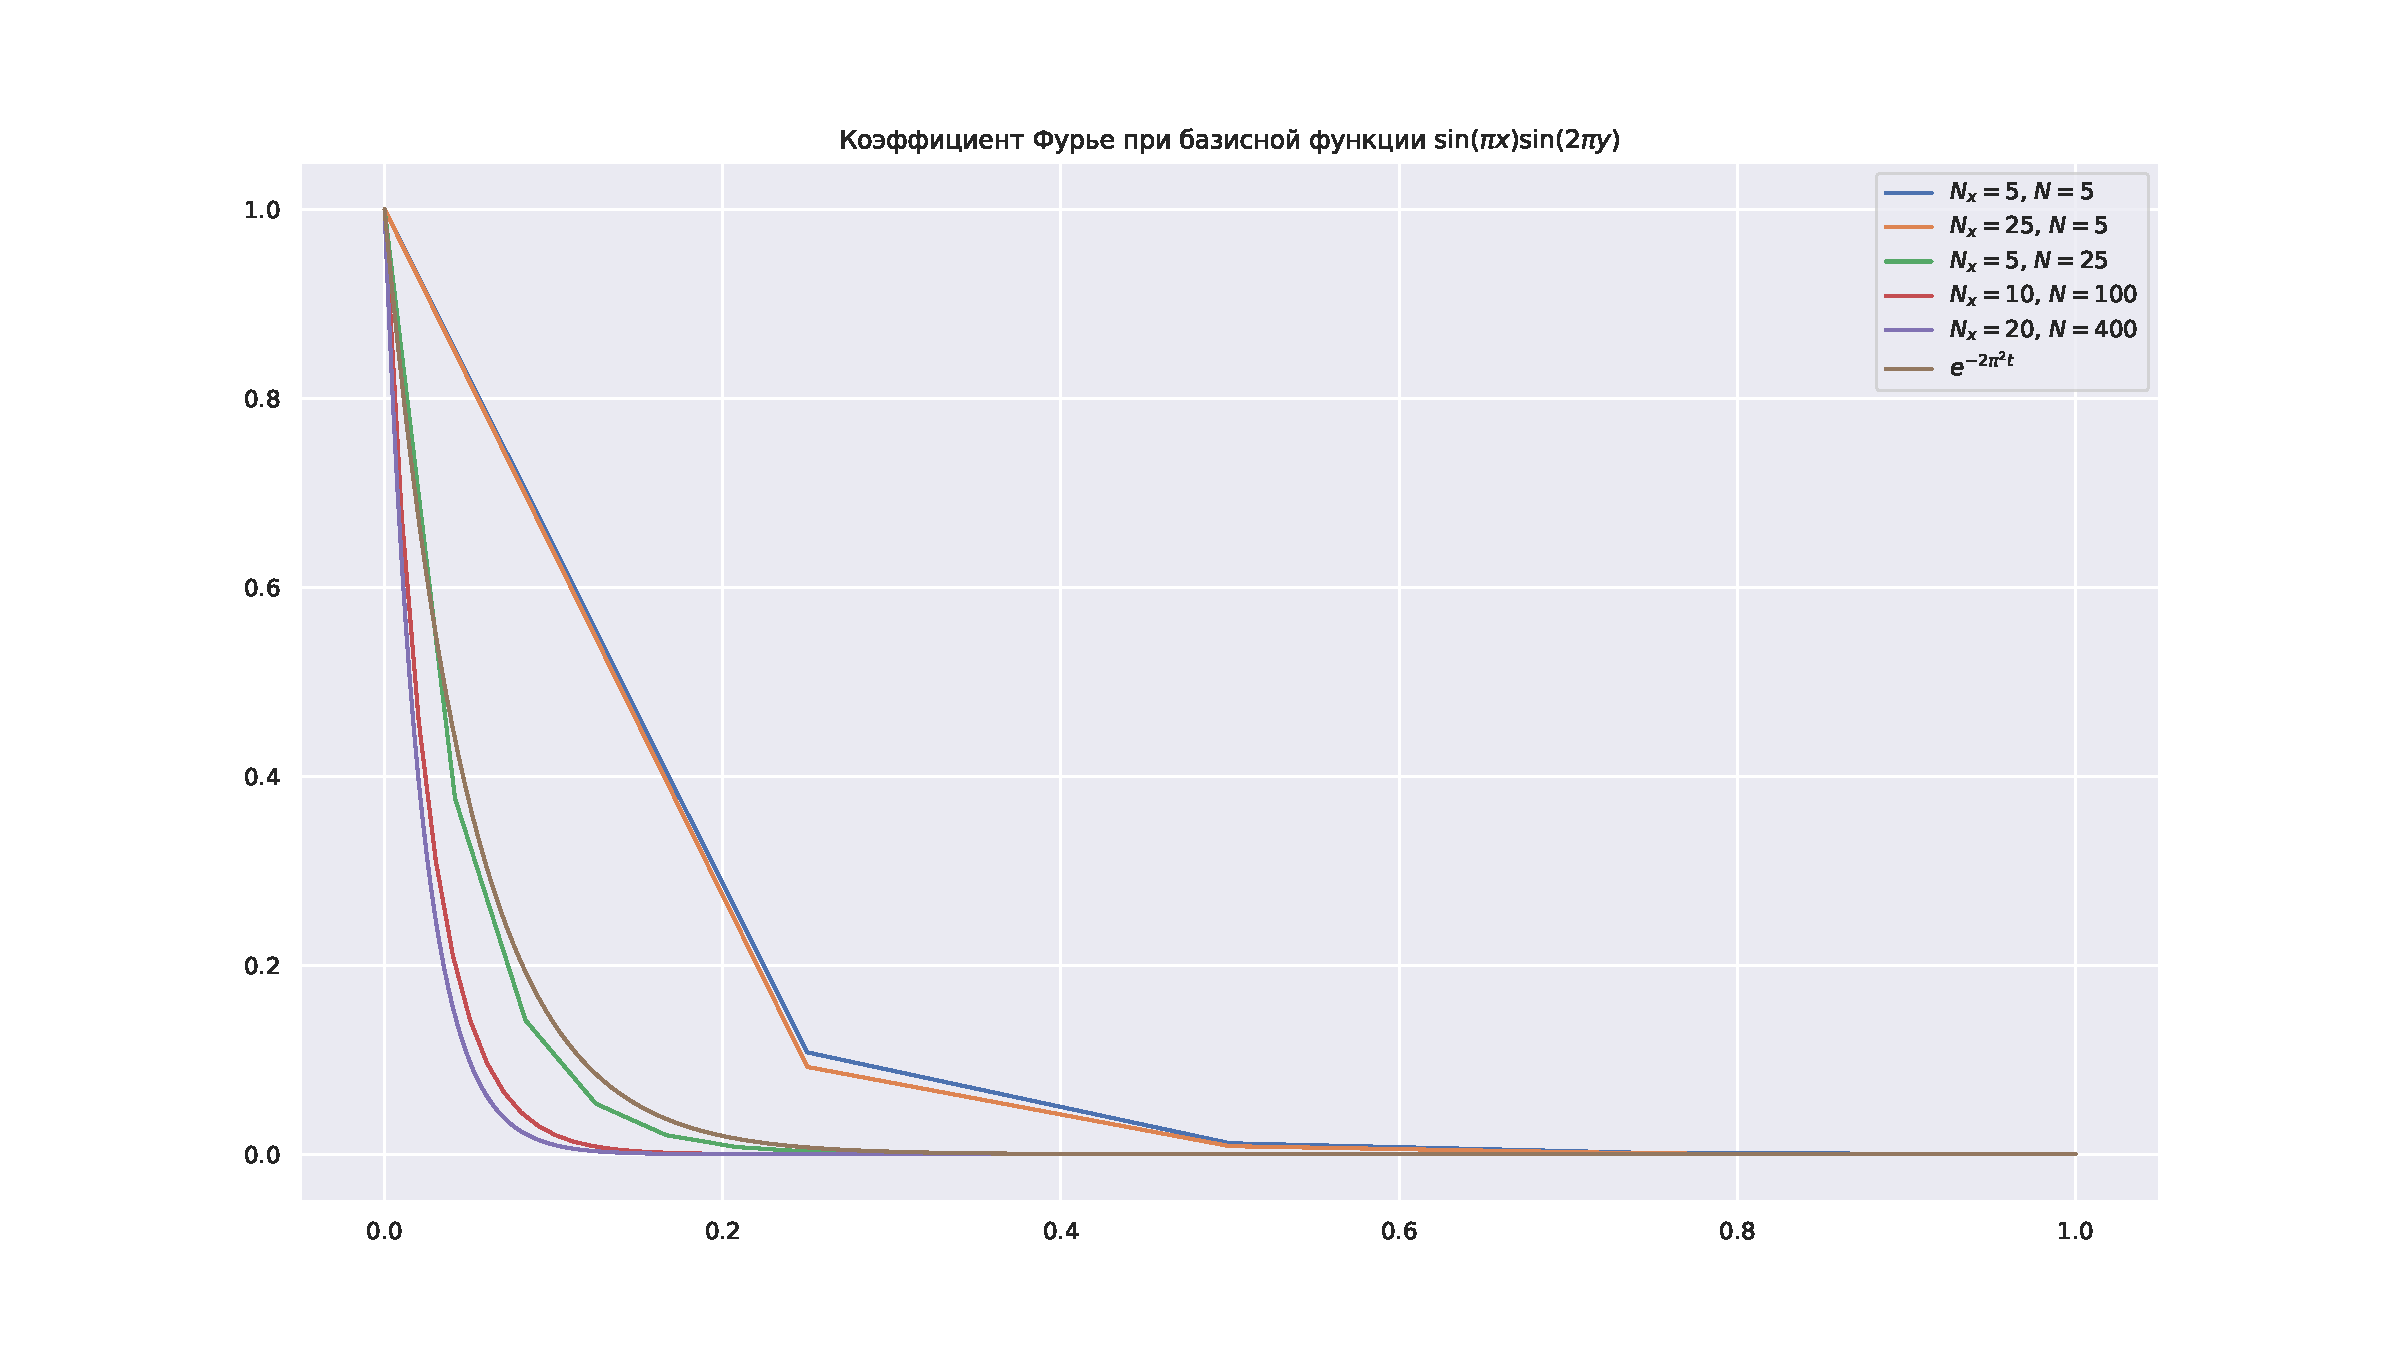
\includegraphics[scale=0.4]{figs/12bf_test.pdf}
    \caption{Задача \ref{diffeq1} при $f = 0$, $u(0, x, y) = \sin \pi n x \sin \pi m y$}
    \label{tbf12}
\end{figure}
\begin{figure}
    \centering
    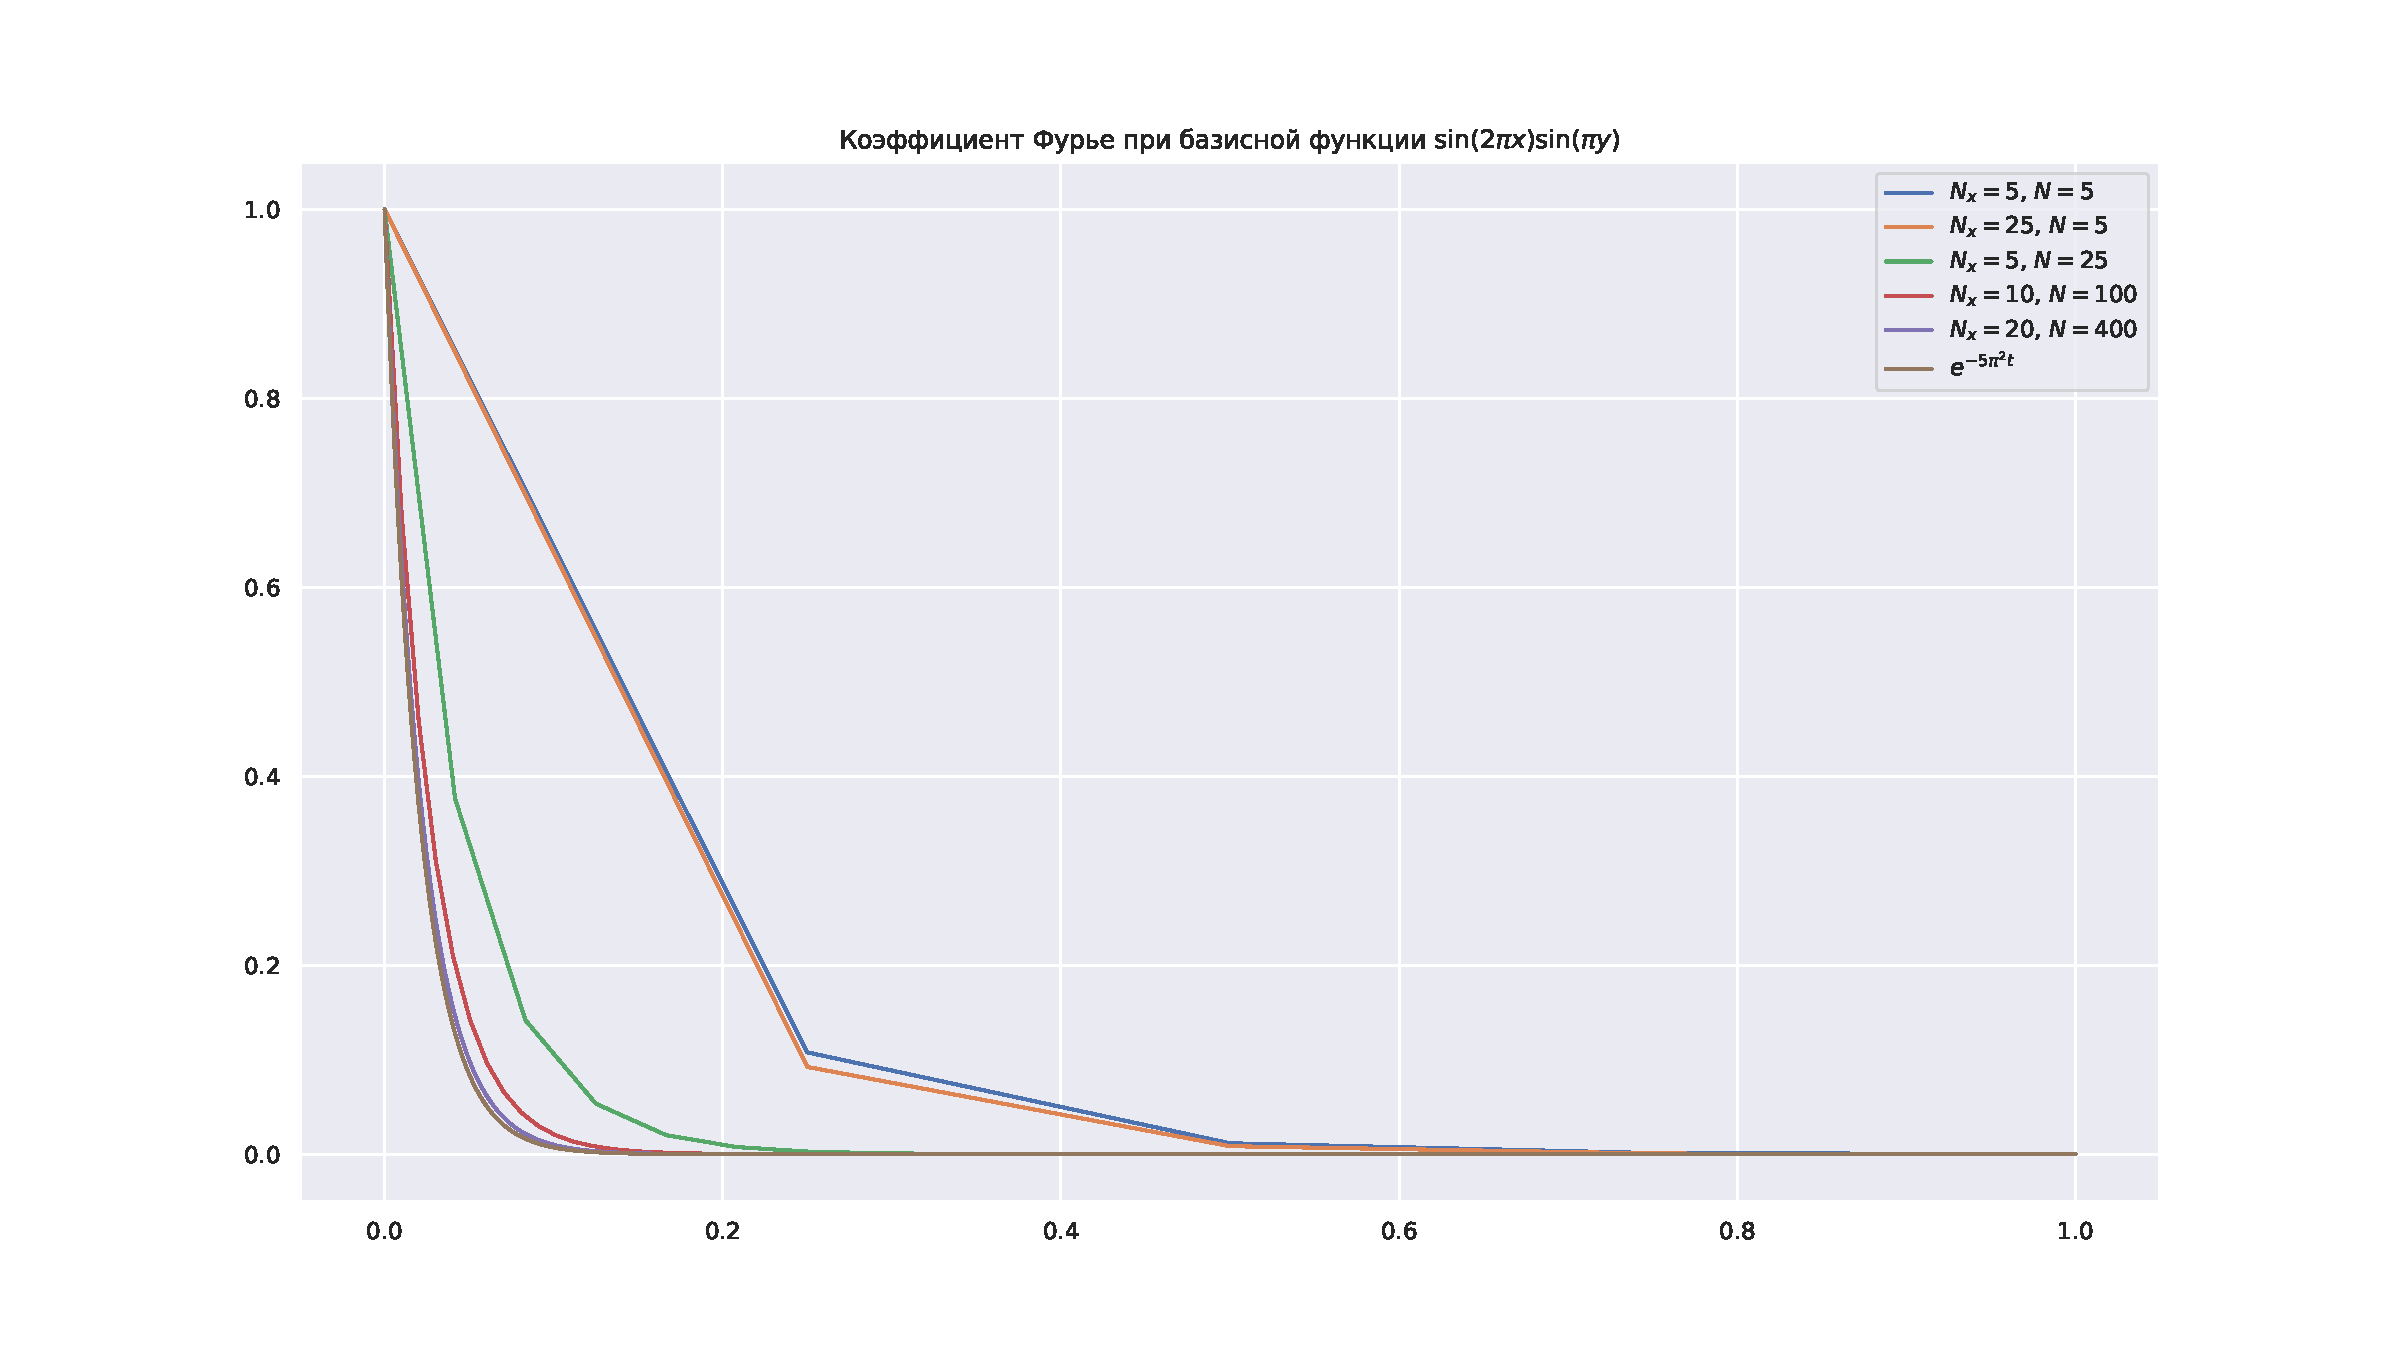
\includegraphics[scale=0.4]{figs/21bf_test.pdf}
    \caption{Задача \ref{diffeq1} при $f = 0$, $u(0, x, y) = \sin \pi n x \sin \pi m y$}
    \label{tbf21}
\end{figure}
\begin{figure}
    \centering
    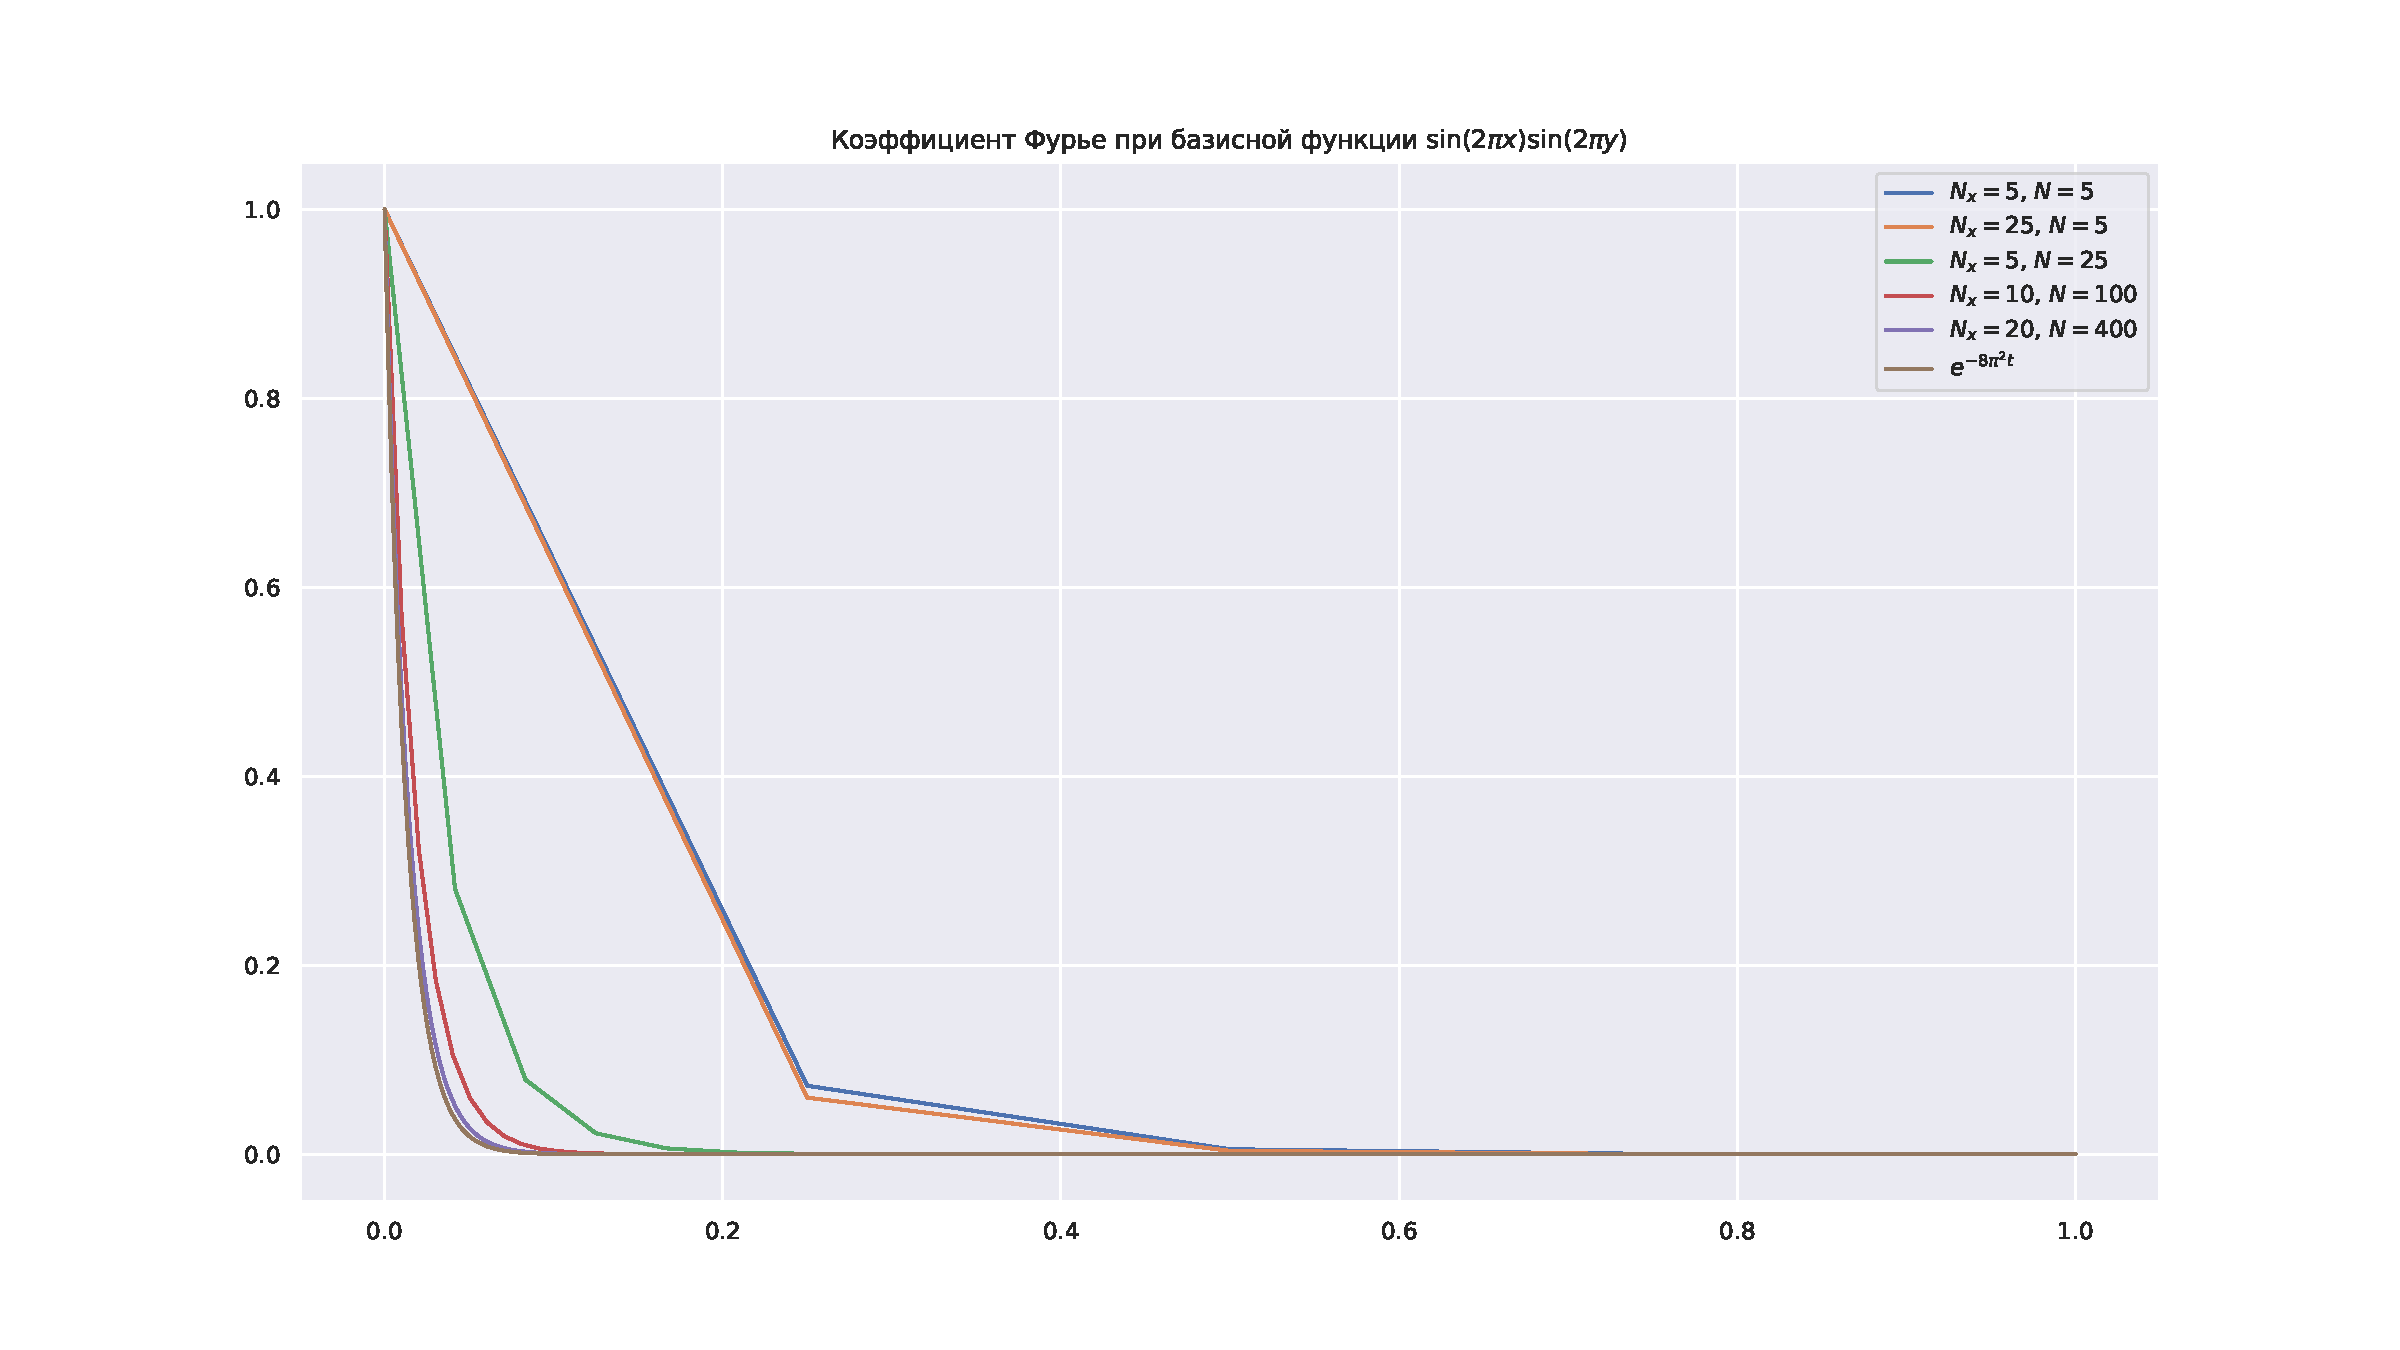
\includegraphics[scale=0.4]{figs/22bf_test.pdf}
    \caption{Задача \ref{diffeq1} при $f = 0$, $u(0, x, y) = \sin \pi n x \sin \pi m y$}
    \label{tbf22}
\end{figure}

\subsection{Ненулевая правая часть.}
Рассмотрим частный случай задачи \ref{diffeq1}, в котором легко угадать решение:
\begin{equation*} 
    u_t(t, x) = u_{xx}(t, x, y) + u_{yy}(t, x, y) + e^{-2 \pi^2 t} \sin \pi x \sin \pi y,
\end{equation*}
краевые условия:
\begin{align*} 
    &u(t, x, y) \big| _{(x ,y) \in \partial \Omega} = 0, \quad \Omega = [0,1] \times [0,1]. \\
    &u(0, x, y) = 0, \quad (x, y) \in \Omega. 
\end{align*}
Тогда видим, что функция
\begin{equation*}
    u(t, x, y) = t e^{-2 \pi^2 t} \sin \pi x \sin \pi y
\end{equation*}
является решением рассматриваемой задачи. Её единственный ненулевой коэффициент Фурье $u_{11}^t = t e^{-2 \pi^2 t}$, с этой функцией мы будем сравнивать численный результат (см. график \ref{tnzf}). 
\begin{figure}
    \centering
    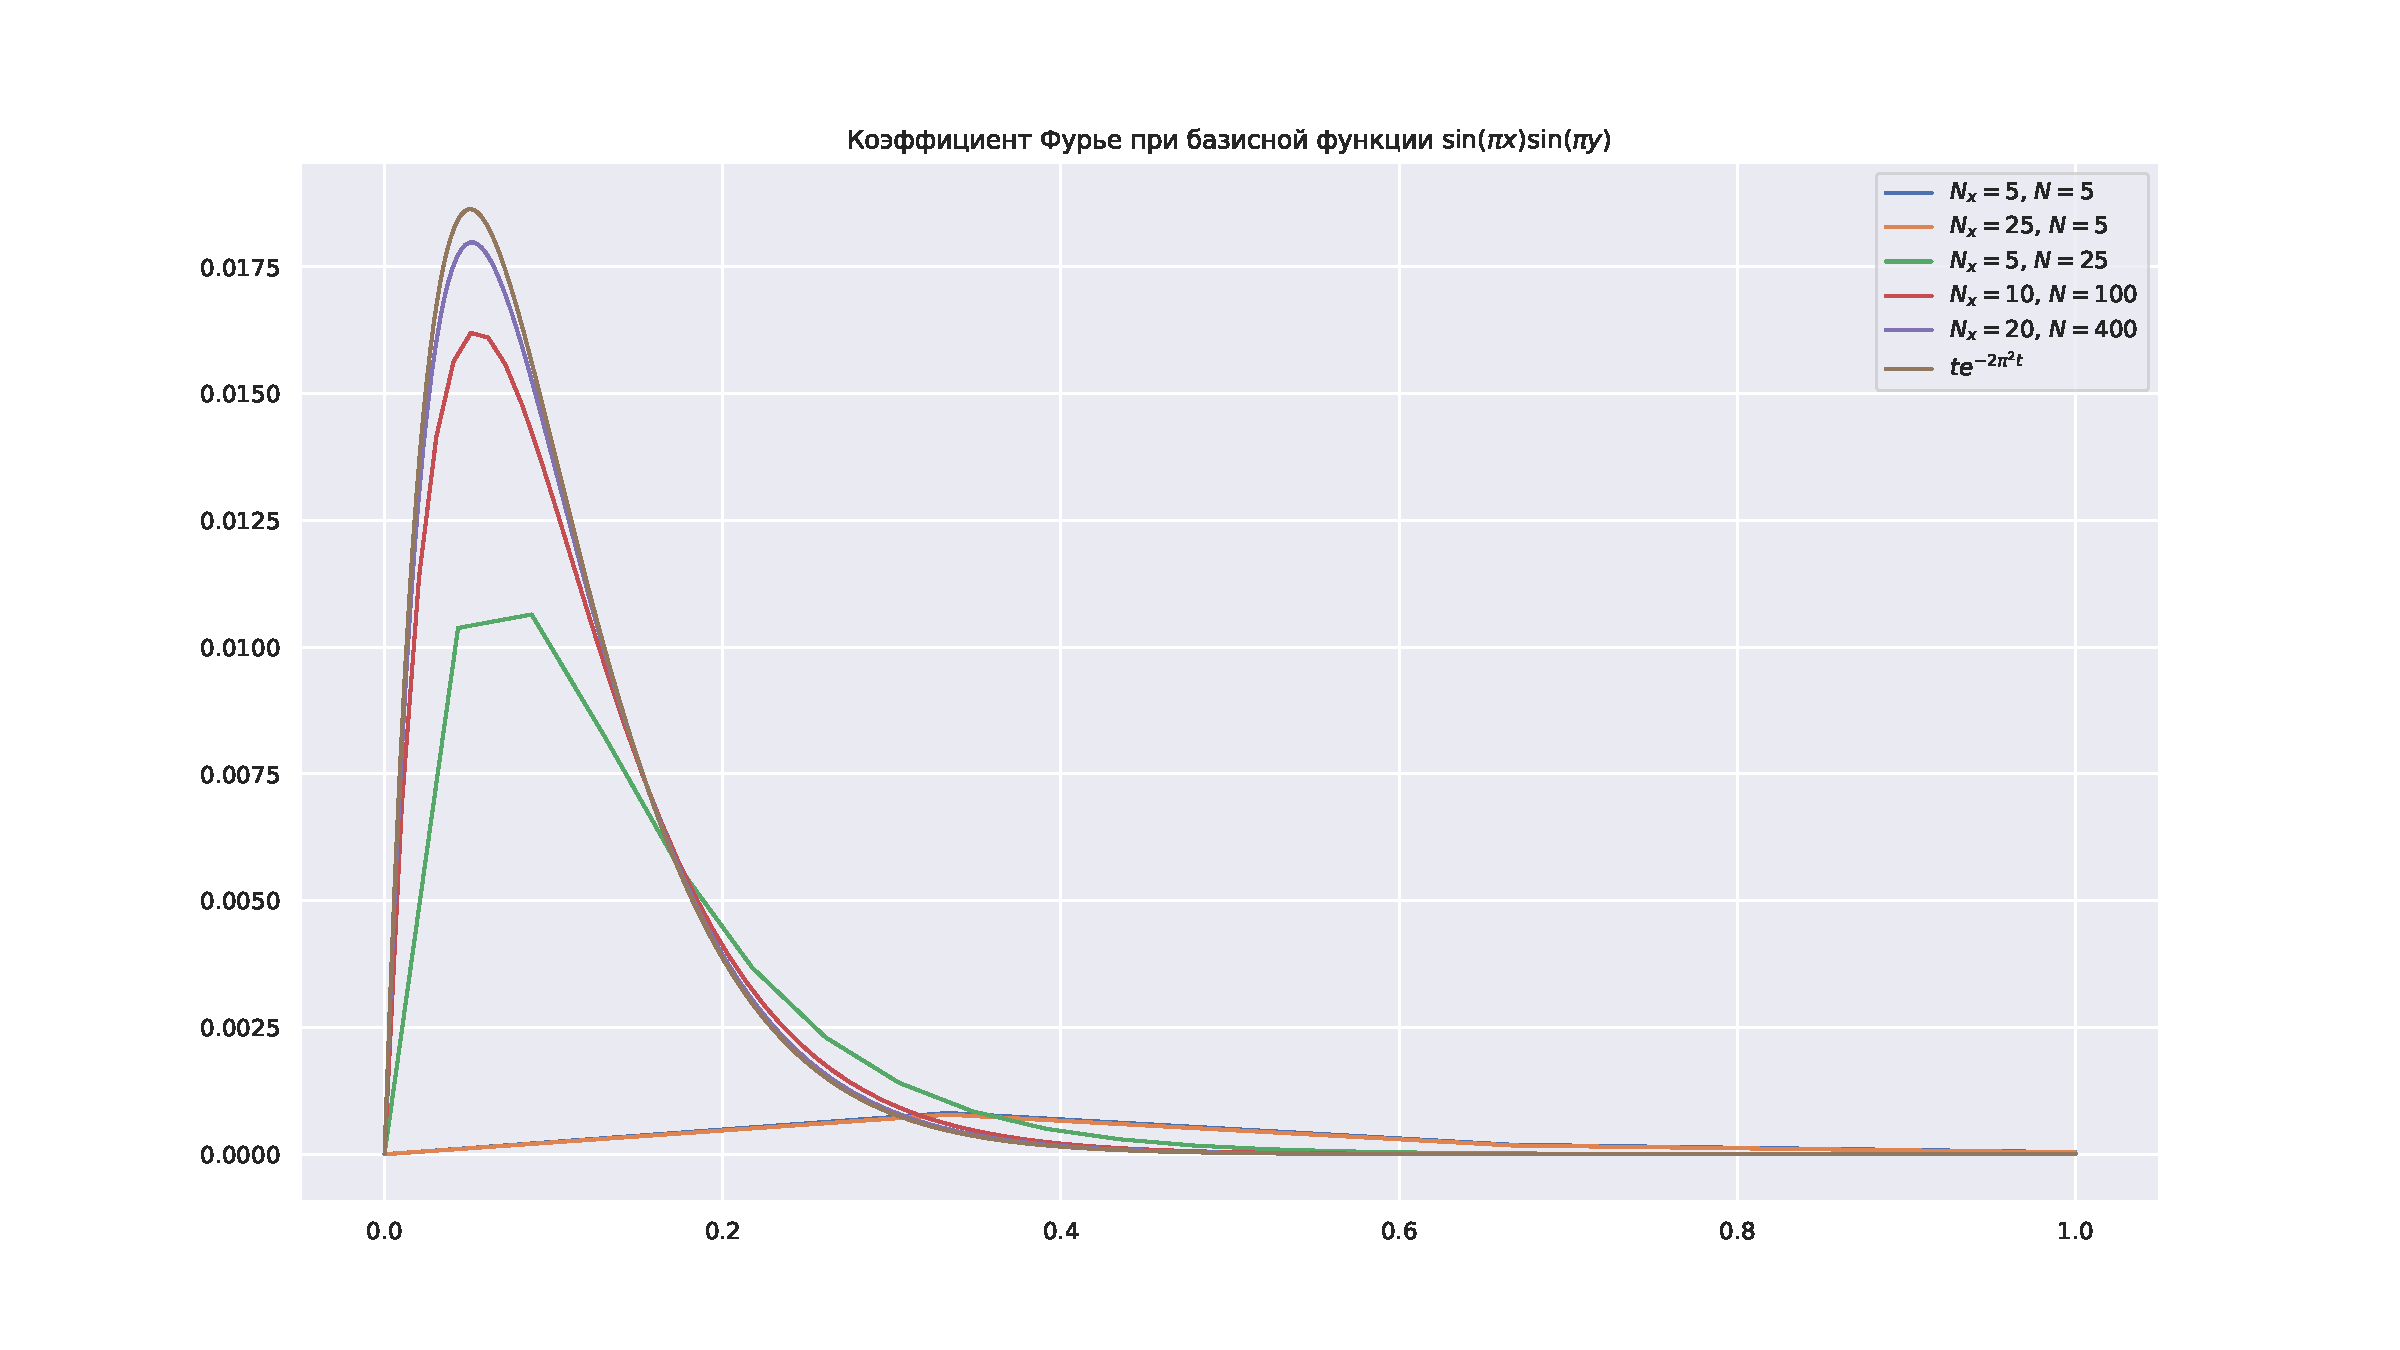
\includegraphics[scale=0.4]{figs/nzf_test.pdf}
    \caption{Задача \ref{diffeq1} при $f = \sin \pi n x \sin \pi m y$, $u(0, x, y) = 0$}
    \label{tnzf}
\end{figure}

\subsection{Скорость сходимости.}
Было проведено две серии тестов скорости сходимости: 
\begin{enumerate}
    \item $(N, N_x, N_y) = \left\{(i, i), \quad i \in \{100, 200, 300, 400, 500\} \right\}$ --- для проверки сходимоти $O(\tau)$.
    \item $(N, N_x, N_y) = \left\{(i^2, i, i), \quad i \in \{10, 20, 30\} \right\}$ --- для проверки сходимоти $O(h_x^2 + h_y^2)$.
\end{enumerate}
Если 
$$\delta(N, N_x, N_y) = \max_{n\leq N, i \leq N_x, j \leq N_y} |u(t_n, x_i, y_j) - u_h(t_n, x_i, y_j)| = O(h_x^2 + h_y^2 + \tau),$$ 
то: 
\begin{enumerate}
    \item при хорошем $h$ (в тесте взято $h_x = h_y = h = \tau  $): \\$ \ln\left(\delta(N, N_x, N_y)\right) \approx \ln(\tau) + \text{const},$
    \item при плохом  $h$ (в тесте взято $h_x = h_y = h = \sqrt{\tau}$): \\$ \ln\left(\delta(N, N_x, N_y)\right) \approx \ln(h) + \text{const}.$
\end{enumerate}
Из графиков \ref{t1} и \ref{t2} видно, что эти условия выполнены. 
\begin{figure}
    \centering
    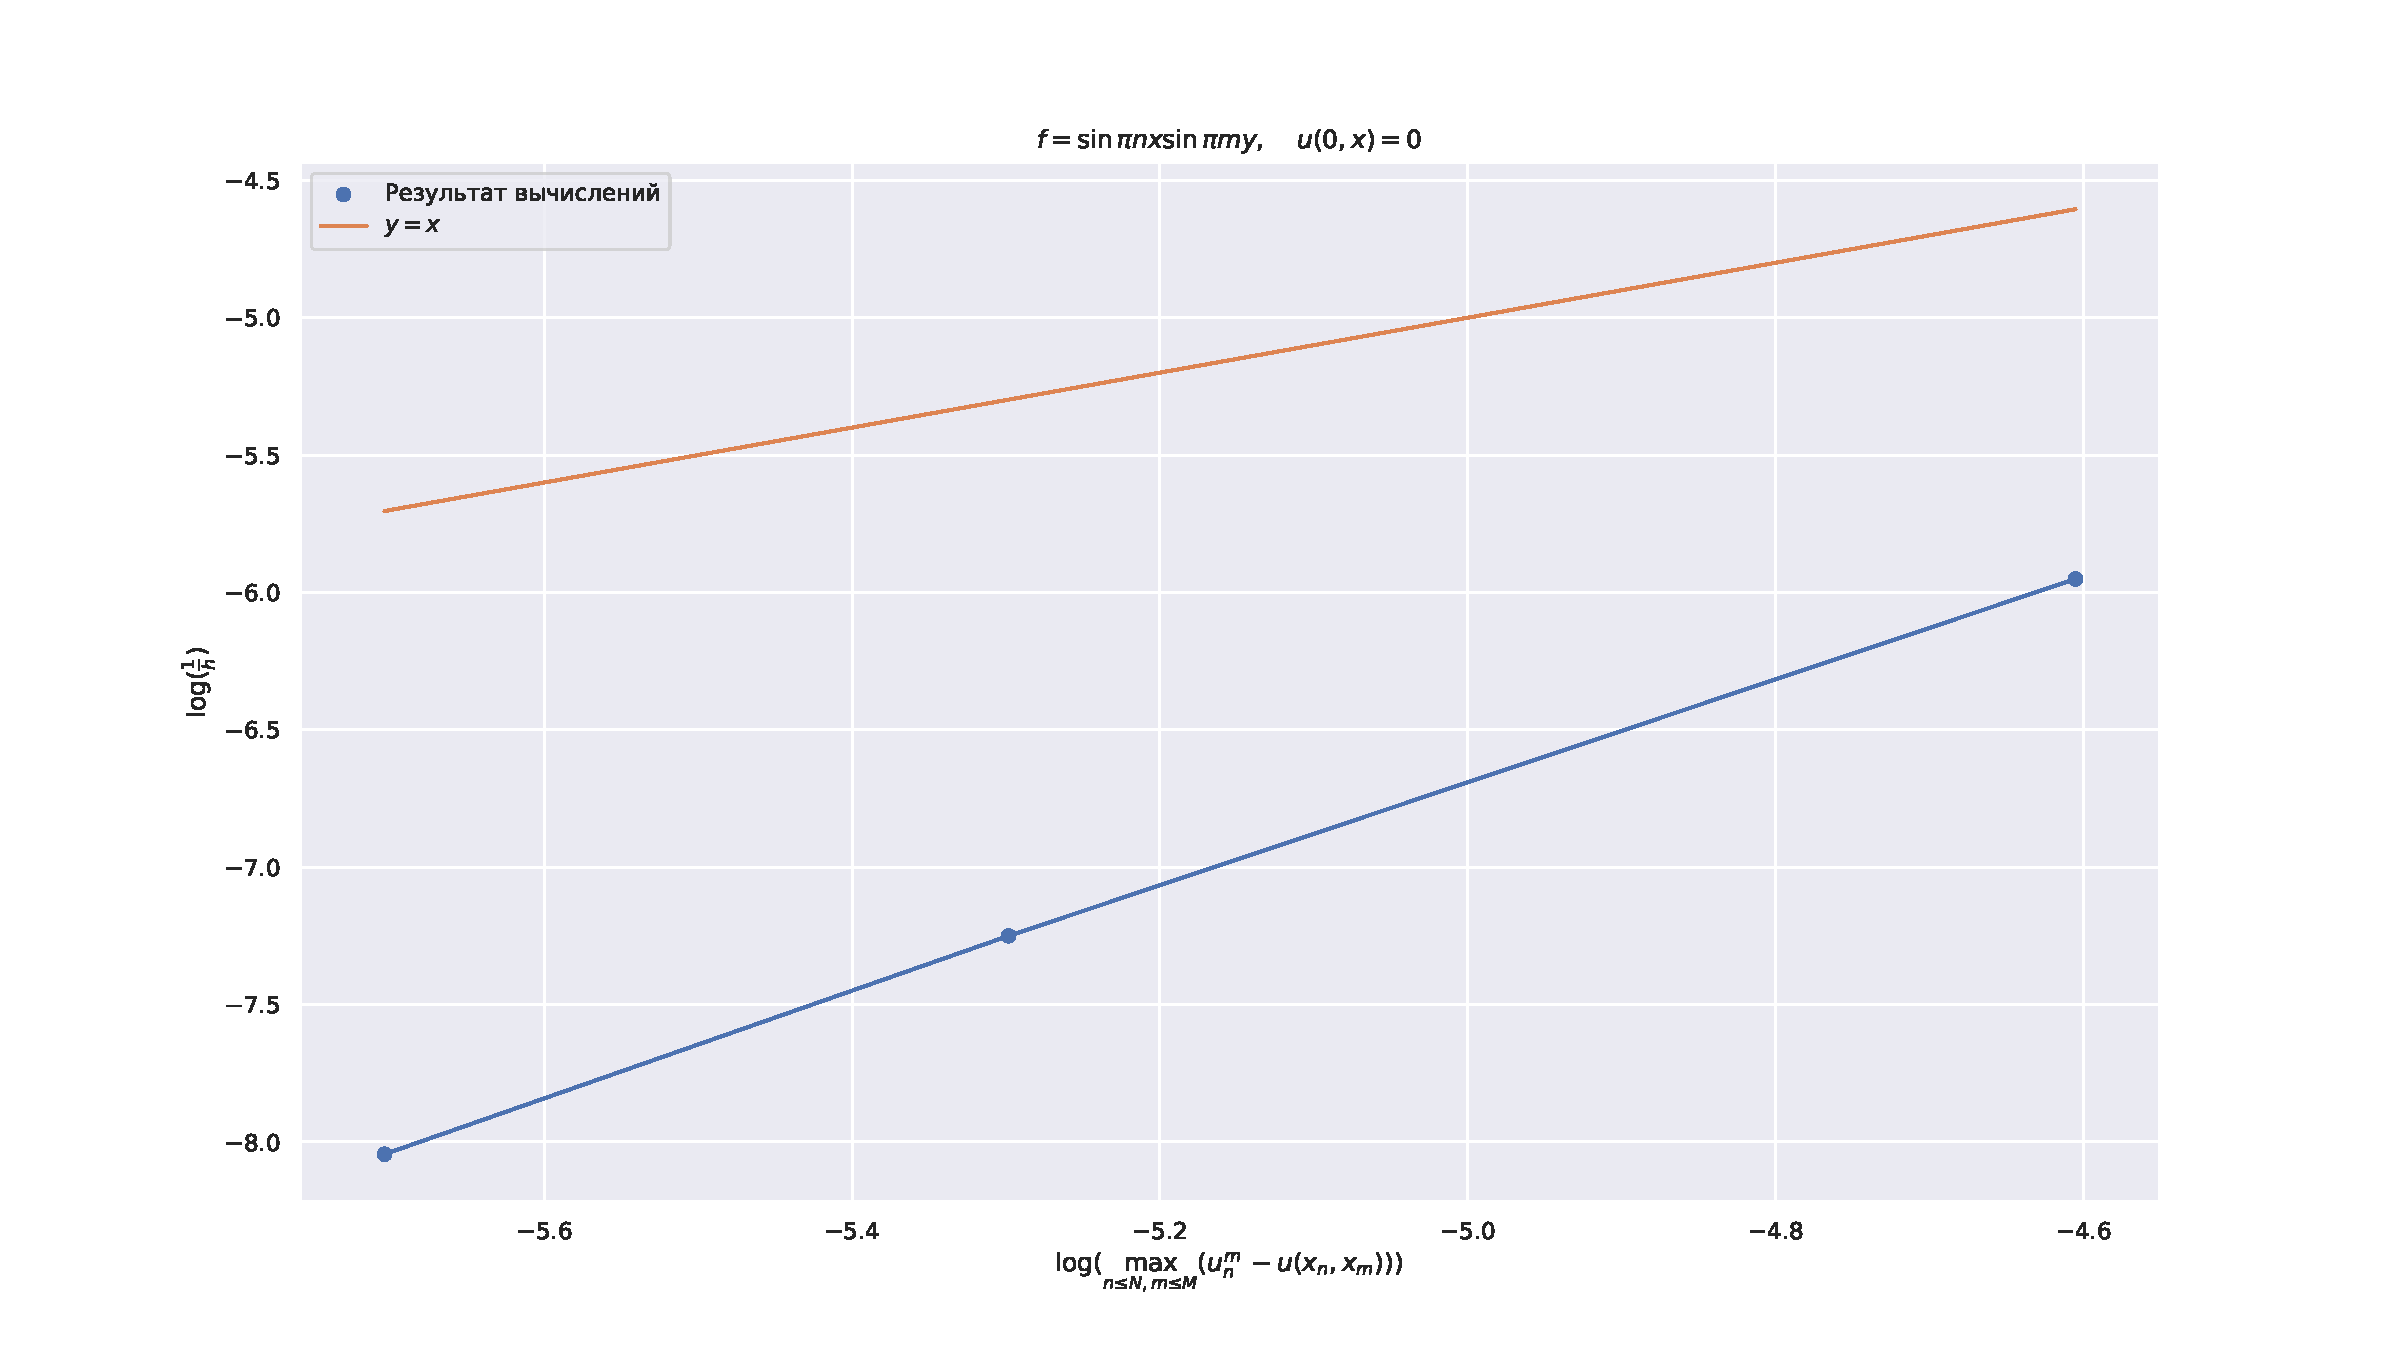
\includegraphics[scale=0.4]{figs/OrderCon1.pdf}
    \caption{Зависимость погрешности от размера сетки в первой серии тестов}
    \label{t1}
\end{figure}

\begin{figure}
    \centering
    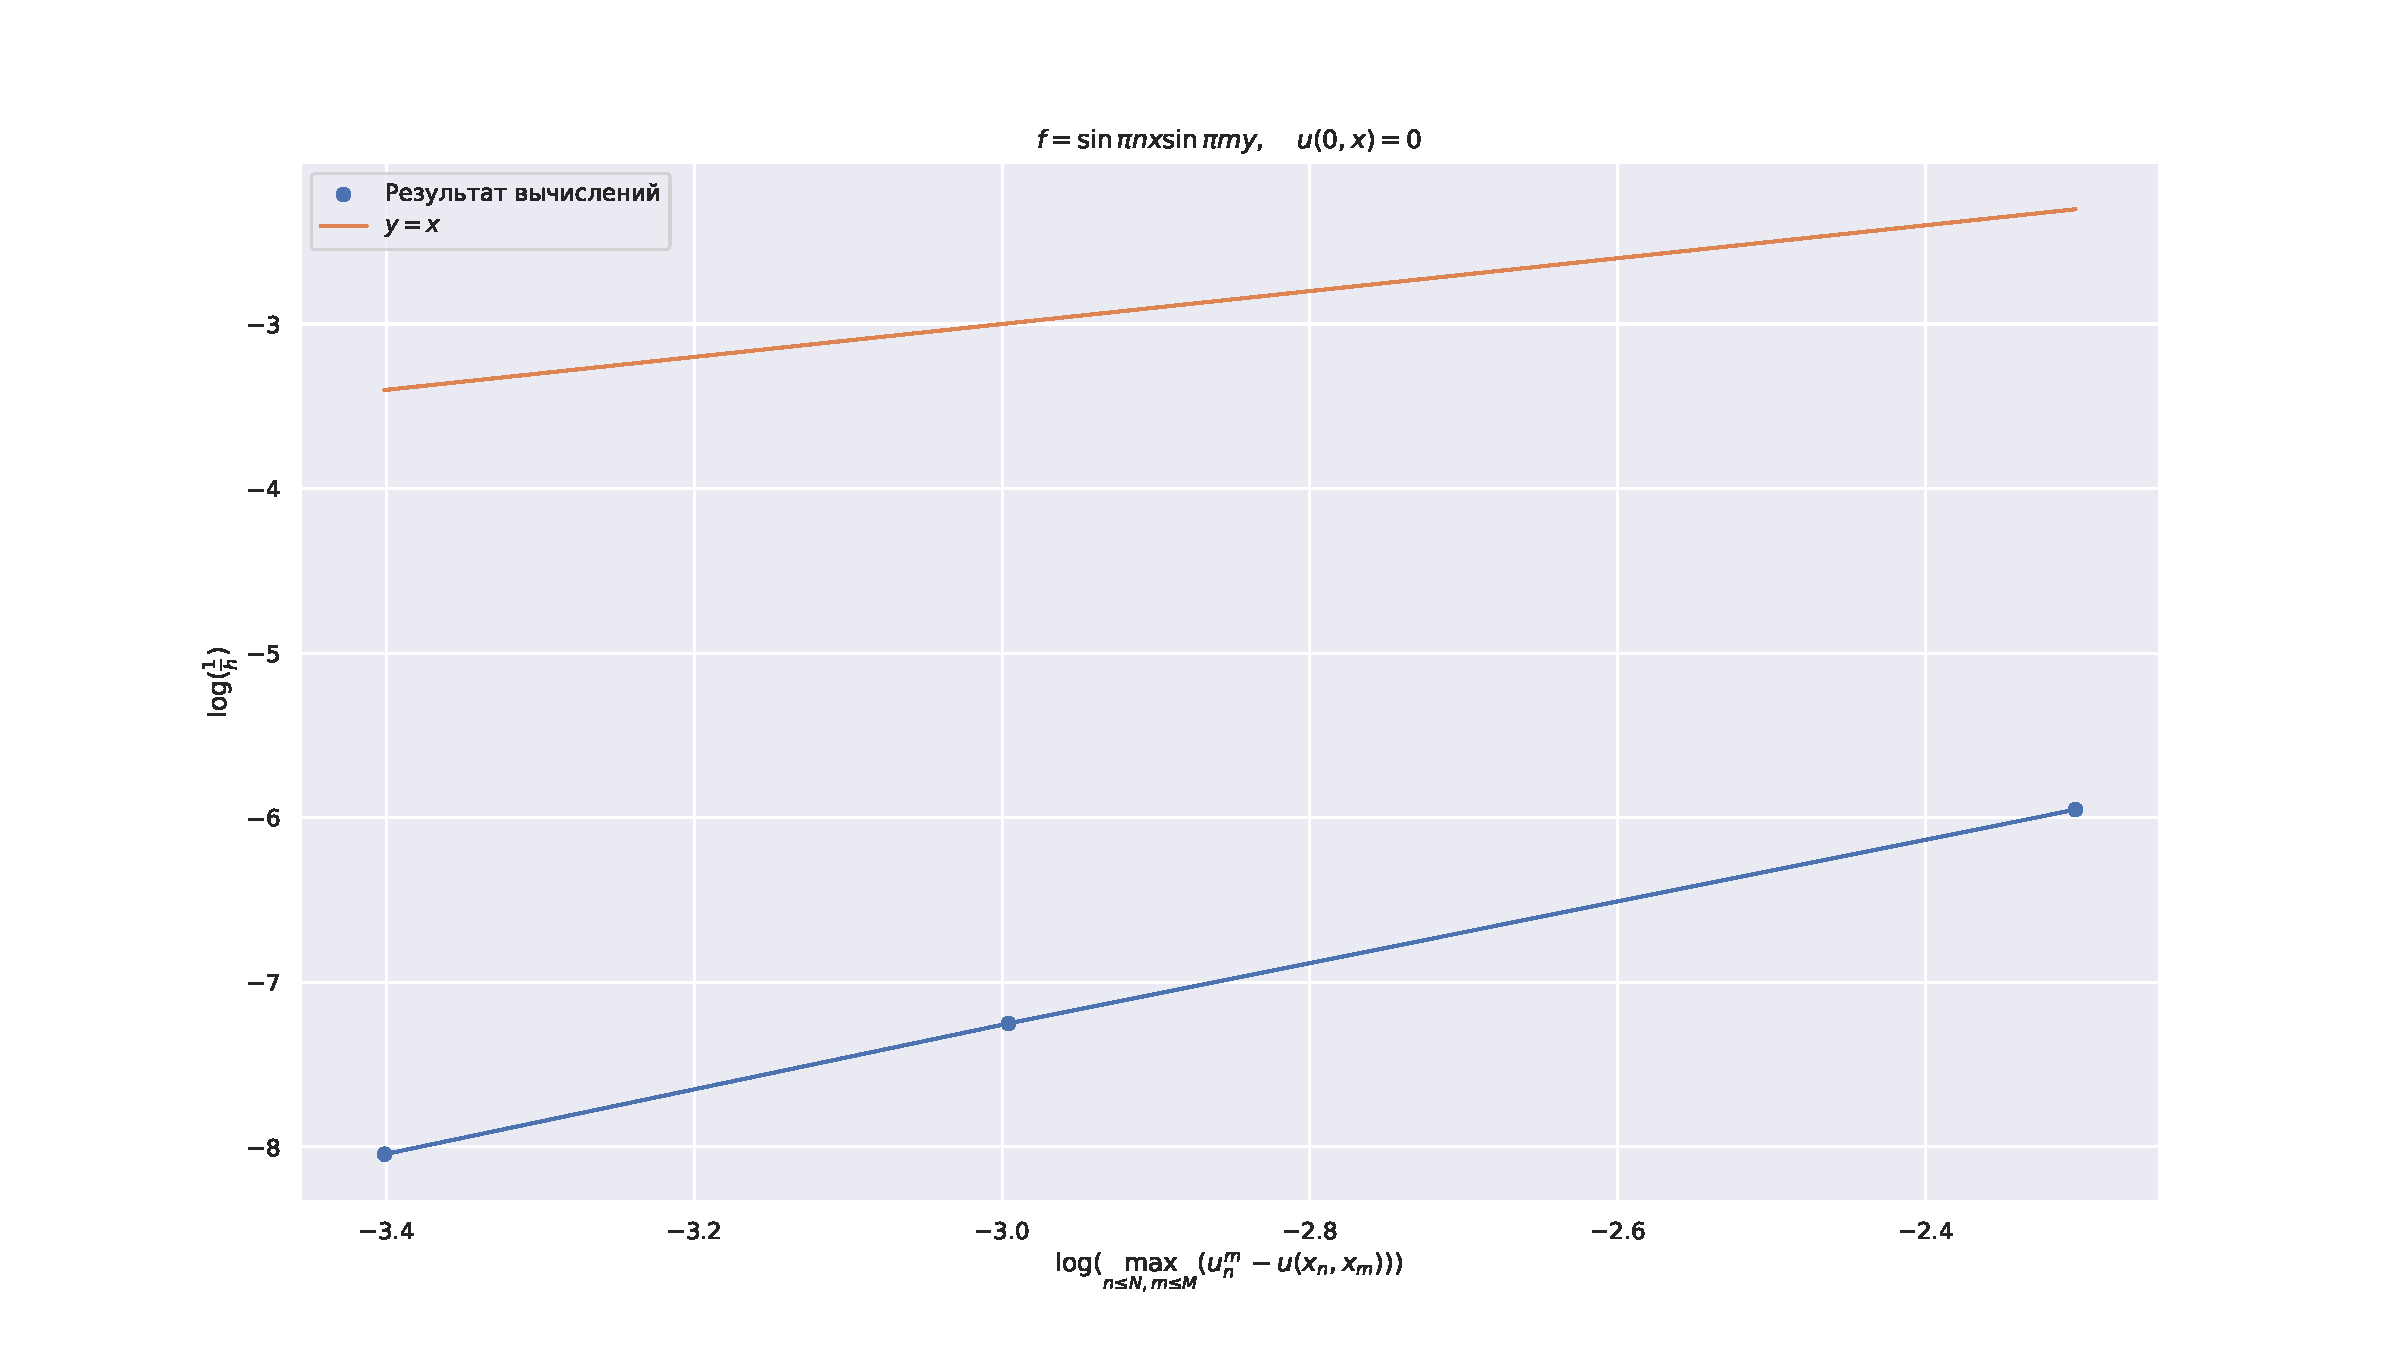
\includegraphics[scale=0.4]{figs/OrderCon2.pdf}
    \caption{Зависимость погрешности от размера сетки во второй серии тестов}
    \label{t2}
\end{figure}

\subsection{Представление ответа в виде гиф-изображения.}
С помощью языка Python для случая ненулевой $f$ было построено три гиф-изображения (см. файл solution\_pict.ipynb):
\begin{enumerate}
    \item Файл error.gif демонстрирует изменение ошибки схемы, по сравнению с аналитическим решением.
    \item Файл numeric\_vs\_analitical.gif демонстрирует динамику численного и аналитического решения (численное решение соответствует красным точкам на графике).
    \item Файл analitical.gif демонстрирует аналитическое решение в динамике.
    \item Файл numerical.gif демонстрирует численное решение в динамике.
\end{enumerate}

 \end{document}